%
%  Network Algorithms - BasicTorrent - Project Report
%
\documentclass[a4paper,12pt,twocolumn]{article}

\usepackage[a4paper]{geometry}
\usepackage[utf8]{inputenc}
\usepackage[T1]{fontenc}
\usepackage{graphicx}
\usepackage{amsmath}
\usepackage{amssymb}
\usepackage{hyperref}
\usepackage{caption}
\usepackage{float}
\usepackage{listings}
\usepackage{subfig}
\usepackage{color}

\newcommand{\sref}[1]{Section~\ref{#1}}
\newcommand{\tref}[1]{Table~\ref{#1}}
\newcommand{\fref}[1]{Figure~\ref{#1}}
\newcommand{\eref}[1]{Equation~\ref{#1}}
\newcommand{\aref}[1]{Appendix~\ref{#1}}

\renewcommand{\figurename}{Fig.}
\renewcommand{\tablename}{Tab.}

\hypersetup{
  colorlinks=true,
  urlcolor=blue,
  linkcolor=blue,
  pdftitle={Network Algorithms - BasicTorrent - Project Report},
  pdfauthor={Uwe Dauernheim <uwe@dauernheim.net>, Alex Averbuch <alex.averbuch@gmail.com>},
  pdfsubject={EP2400 - Network Algorithms}
}

\captionsetup{
  justification=centering,
  width=0.40\textwidth,
  font=small,
  labelfont=bf,
%  format=hang
}

\captionsetup[subfloat]{
  justification=centering,
  width=0.22\textwidth,
  font=footnotesize,
  labelfont=bf,
%  format=hang
}

\geometry{
  vmargin={35mm,35mm},
  hmargin={25mm,25mm}
}

\hyphenpenalty=10000

%%%%%%%%%%%%%%%%%%%%%%%%%%%%%%%%%%%%%%%%%%%%%%%%%%%%%%%%%%%%%%%%%%%%%%%%
\title{
  \bf Case Study about Basic Torrent \\ \ using SICSIM \\ 
  \small{\bf Project Report}}
\author{
  \begin{tabular}[t]{c@{\extracolsep{8em}}c} 
    Uwe Dauernheim\textsuperscript{†} & 
    Alex Averbuch\textsuperscript{†} \\
    uwe@dauernheim.net & alex.averbuch@gmail.com \\
  \end{tabular}
  \\ \\
  \textsuperscript{†} EP2400 - Network Algorithms
}
%%%%%%%%%%%%%%%%%%%%%%%%%%%%%%%%%%%%%%%%%%%%%%%%%%%%%%%%%%%%%%%%%%%%%%%%
%%\tiny
%%\scriptsize
%%\footnotesize
%%\small
%%\normalsize
%%\large
%%\Large
%%\huge
%%\Huge

\hyphenation{SICSIM}

\begin{document}

\maketitle
%\onecolumn
%\tableofcontents
%\pagebreak
%\twocolumn

\section{Introduction}
\label{sec:introduction}
As part of this project a simplified, centralized version of BitTorrent was developed and evaluated using \emph{SICSIM}\footnote{\url{http://www.sics.se/~amir/sicsim/}}, a Java-based network simulator.

This report briefly outlines the protocol in \sref{sec:protocol}, introduces important definitions in \sref{sec:definitions}, describes the experiments performed in \sref{sec:experiments}, reasons about the results in \sref{sec:results_analysis}, and concludes with a brief discussion in \sref{sec:discussion}.

\section{Protocol}
\label{sec:protocol}
The protocol under analysis is loosely based on BitTorrent, although greatly simplified. 

As in BitTorrent, the protocol employs a centralized Tracker, but in this case the Tracker maintains a global view of all peers' state.

Piece selection and seeder selection strategies are random and performed by the Tracker only.

Peers send requests for pieces to the Tracker. The Tracker then responds with instructions comprising of: a random piece (that peer does not already have) to download next, and the address of the seeder for that piece.

Peers may not download multiple pieces from the same seeder in parallel.

\section{Definitions}
\label{sec:definitions}

Before presenting the experiments and results, it is important to define a number of concepts.
The following definitions are provided as a reference for \sref{sec:experiments} and \sref{sec:results_analysis}.

In all experiments the simulated network links had a latency of:
\begin{eqnarray}
\label{eqn:t_network}
  T_{\text{network}}=6 \pm 3 \text{ms}
\end{eqnarray}

Churn defines the amount of peers joining/leaving the network, and the frequency of these events:
\begin{eqnarray}
\label{eqn:churn}
  \text{Churn} = 0\% \dots 100\%
\end{eqnarray}

In this protocol, files are divided into pieces. The size of each piece is given by:
\begin{eqnarray}
\label{eqn:piece_size}
  \text{Size}_{\text{piece}}= \frac{\text{Size}_{\text{file}}}{\text{Count}_{\text{pieces}}}
\end{eqnarray}

In this protocol a peer's upload bandwidth is statically and evenly shared across its upload slots. The time required to simply transfer one piece between two peers is dependent on several factors, including piece size and the upload bandwidth available to one slot. This ignores any overhead incurred by protocol messages and is given by:
\begin{eqnarray}
\label{eqn:t_transfer}
  T_{\text{transfer}} = \frac{\text{Size}_{\text{piece}}}{\left(\frac{\text{BW}_{\text{up}}}{\text{Slots}_{\text{up}}}\right)}
\end{eqnarray}

The time required to perform all protocol interactions that support a piece transfer can be significant. There are six messages, including: sending request to/from tracker, performing handshake with seeder, initiating download from seeder, and receiving complete notification from seeder. This ignores any processing time between messages and also ignores the time needed to actually transfer the piece. It is given by:
\begin{eqnarray}
\label{eqn:t_protocol}
  T_{\text{protocol}} = 6 \times T_{\text{network}}
\end{eqnarray}

The time required to download a piece, excluding any processing time but including all protocol messages and the actual piece transfer, is given by:
\begin{eqnarray}
\label{eqn:t_download}
  T_{\text{download}}=T_{\text{protocol}} + T_{\text{transfer}}
\end{eqnarray}

Slot utilization defines how many of its available upload slots a peer is using. It is given by:
\begin{eqnarray}
\label{eqn:utilization_slot}
  \text{Util}_{\text{slots}} = 0\% \dots 100\%
\end{eqnarray}

It is unlikely that a peer is always utilizing all of it's available upload bandwidth. The amount of upload bandwidth a peer is utilizing at any given time is given by:
\begin{eqnarray}
\label{eqn:bandwidth_peer}
  \text{BW}_{\text{peer}}=\text{BW}_{\text{up}} \times \text{Util}_{\text{slots}}
\end{eqnarray}

The benefit of peer-to-peer systems is realized by harnessing the resources of all peers. In this protocol, as more peers seed file pieces, the available global system bandwidth ($\text{BW}_{\text{system}}$) increases. However, it is difficult to accurately describe how $\text{BW}_{\text{system}}$ changes with time without simplifying the problem.

Assume that: pieces are uniformly distributed across all peers as soon as possible, all pieces are equally available in the network, and peers equally share the load of seeding as soon as possible.
Given these assumptions this basic equation can be used to model the change in $\text{BW}_{\text{system}}$ with time:
\begin{eqnarray}
\label{eqn:bandwidth_system}
  T &=& i \times T_{\text{download}}\nonumber \\
  \text{BW}_{\text{system}}^{T_0} &=& \text{BW}_{\text{up}} \nonumber \\
  \text{BW}_{\text{system}}^{T} &=& (\text{Slots}_{\text{up}} + 1) \times \text{BW}_{\text{system}}^{T-1} \nonumber \\
\end{eqnarray}


\section{Experiments}
\label{sec:experiments}
Experiments were carried out to determine how various protocol parameters affect performance. This section details these experiments.

\subsection{Slot Count}
\label{subsec:slots}
$\text{Slots}_{\text{up}}$ and $\text{Slots}_{\text{down}}$ dictate how many pieces a peer can upload/download simultaneously.

These parameters were varied to gauge the effect they had on piece dissemination.

Experiment settings can be seen in \tref{tab:slots}.

\begin{table}[!htbp]
\centering
\footnotesize
\begin{tabular}{lll}
\textbf{Parameter} & \textbf{Value} \\
Churn & 0\% \\
Network Size & 100 \\
Peer Inter-arrival Time & 10 \\
$\text{BW}_{\text{up}}$ & 32 \\
$\text{BW}_{\text{down}}$ & Unlimited \\
$\text{Count}_{\text{pieces}}$ & 10 \\
$\text{Size}_{\text{piece}}$ & 64 \\
$\text{Slots}_{\text{up}}$ & 1-12 \\
$\text{Slots}_{\text{down}}$ & 1-12 \\
\end{tabular}
\captionof{table}{Experiment Settings - Slot Count}
\label{tab:slots}
\end{table}

Peers did not begin to download pieces until all peers had joined the network.
This was done in an attempt to eliminate all variables from the experiment, other than the slot count.

Data collection began as soon as the last peer joined the network.

\subsection{Network Size}
\label{subsec:network_size}
The number of peers in the system was varied. Experiment settings can be seen in \tref{tab:network_size}.

\begin{table}[ht!]
\centering
\footnotesize
\begin{tabular}{lll}
\textbf{Parameter} & \textbf{Value} \\
Churn & 0\% \\
Network Size & 1-1000 \\
Peer Inter-arrival Time & 10 \\
$\text{BW}_{\text{up}}$ & 128 \\
$\text{BW}_{\text{down}}$ & Unlimited \\
$\text{Count}_{\text{pieces}}$ & 10 \\
$\text{Size}_{\text{piece}}$ & 64 \\
$\text{Slots}_{\text{up}}$ & 4 \\
$\text{Slots}_{\text{down}}$ & 4 \\
\end{tabular}
\captionof{table}{Experiment Settings - Network Size}
\label{tab:network_size}
\end{table}

Peers did not begin to download pieces until all peers had joined the network. 
This was done in an attempt to eliminate all variables from the experiment, other than the number of peers.
If this method had not been used, time taken to complete the experiment would have depended almost entirely on the time required for every peer to join the network.

Data collection began as soon as the last peer joined the network.

\subsection{Upload Bandwidth}
\label{subsec:upload_bandwidth}
Clearly, peers' upload bandwidth has an effect on how fast pieces can be exchanged in the network. 
To explore effects related the upload bandwidth, this parameter was varied and experiments were performed.

Experiment settings can be seen in \tref{tab:upload_bandwidth}.

\begin{table}[!htbp]
\centering
\footnotesize
\begin{tabular}{lll}
\textbf{Parameter} & \textbf{Value} \\
Churn & 0\% \\
Network Size & 100 \\
Peer Inter-arrival Time & 10 \\
$\text{BW}_{\text{up}}$ & 32-1024 \\
$\text{BW}_{\text{down}}$ & Unlimited \\
$\text{Count}_{\text{pieces}}$ & 10 \\
$\text{Size}_{\text{piece}}$ & 64 \\
$\text{Slots}_{\text{up}}$ & 4 \\
$\text{Slots}_{\text{down}}$ & 4 \\
\end{tabular}
\captionof{table}{Experiment Settings - Upload Bandwidth}
\label{tab:upload_bandwidth}
\end{table}

Peers did not begin to download pieces until all peers had joined the network. 
This was done in an attempt to eliminate all variables from the experiment, other than the upload bandwidth.

Data collection began as soon as the last peer joined the network.

\subsection{Piece Count}
\label{subsec:piece_count}
Tests were performed to research the effects of varying $\text{Count}_{\text{pieces}}$. Note that $\text{Size}_{\text{file}}$ is fixed in these experiments, so $\text{Size}_{\text{piece}}$ is given by \eref{eqn:piece_size}.

These tests were performed to identify what affects $\text{Count}_{\text{pieces}}$ has on the amount of piece transfers that can be performed in parallel, and the progress of the protocol in general.

Experiment settings can be seen in \tref{tab:piece_count}.

\begin{table}[!htbp]
\centering
\footnotesize
\begin{tabular}{lll}
\textbf{Parameter} & \textbf{Value} \\
Churn & 0\% \\
Network Size & 100 \\
Peer Inter-arrival Time & 10 \\
$\text{BW}_{\text{up}}$ & 64 \\
$\text{BW}_{\text{down}}$ & Unlimited \\
$\text{Count}_{\text{pieces}}$ & 600, 1200, 2400 \\
$\text{Size}_{\text{piece}}$ & 1-50 \\
$\text{Slots}_{\text{up}}$ & 4 \\
$\text{Slots}_{\text{down}}$ & 4 \\
\end{tabular}
\captionof{table}{Experiment Settings - Piece Count}
\label{tab:piece_count}
\end{table}

Peers did not begin to download pieces until all peers had joined the network. 
This was done in an attempt to eliminate all variables from the experiment, other than the upload bandwidth.

Data collection began as soon as the last peer joined the network.

\subsection{Churn}
\label{subsec:churn}
The amount of churn present in the system was varied.  The experiments were performed using reliable seeder: Initial seeder never leaves or fails. Experiment settings can be seen in \tref{tab:churn}.

\begin{table}[!htbp]
\centering
\footnotesize
\begin{tabular}{lll}
\textbf{Parameter} & \textbf{Value} \\
Churn & 0\%-70\% \\
Network Size & 100 \\
Peer Inter-arrival Time & 10 \\
$\text{BW}_{\text{up}}$ & 64 \\
$\text{BW}_{\text{down}}$ & Unlimited \\
$\text{Count}_{\text{pieces}}$ & 10 \\
$\text{Size}_{\text{piece}}$ & 64 \\
$\text{Slots}_{\text{up}}$ & 4 \\
$\text{Slots}_{\text{down}}$ & 4 \\
\end{tabular}
\captionof{table}{Experiment Settings - Churn}
\label{tab:churn}
\end{table}

Peers began to download pieces as soon as they joined the network and data collection began as soon as the first peer joined the network.
This was done in an attempt to simulate a real-world scenario.

\subsection{Leaving Seeders}
\label{subsec:leaving_seeders}
Tests were performed to research the effects of varying the amount of time that a peer stays in the network after downloading all pieces. This attempts to simulate reality, where downloaders often only connect to the network for as long as they have something to gain. This experiment is intended to highlight the protocol's reliance on the ``good will'' of peers.

The amount of time a peer remains in the network after becoming a seeder ($T_{\text{seeding}}$) was varied. After this predefined time, the seeding peers left the network.

Experiments were performed using an unreliable initial seeder: Initial seeder may leave or fail, to simulate a more realistic scenario. Experiment settings can be seen in \tref{tab:leaving_seeders}.

\begin{table}[!htbp]
\centering
\footnotesize
\begin{tabular}{lll}
\textbf{Parameter} & \textbf{Value} \\
Churn & 0\% \\
Network Size & 100 \\
Peer Inter-arrival Time & 10 \\
$\text{BW}_{\text{up}}$ & 64 \\
$\text{BW}_{\text{down}}$ & Unlimited \\
$\text{Count}_{\text{pieces}}$ & 10 \\
$\text{Size}_{\text{piece}}$ & 64 \\
$\text{Slots}_{\text{up}}$ & 4 \\
$\text{Slots}_{\text{down}}$ & 4 \\
$T_{\text{seeding}}$ & 0-500 \\
\end{tabular}
\captionof{table}{Experiment Settings - Leaving Seeders}
\label{tab:leaving_seeders}
\end{table}

Peers began to download pieces as soon as they joined the network. Data collection began as soon as the first peer joined the network.

\section{Results \& Analysis}
\label{sec:results_analysis}

After carrying out the experiments, the results were analyzed.

This section details the results and attempts to reason about each observation.

\subsection{Slot Count - Static Download}
\label{subsec:slots_results_static_download}

In general, it is most beneficial if a piece can be disseminated among the peers as soon as possible. This idea is formalized by \eref{eqn:bandwidth_system}.

When pieces are disseminated more quickly $\text{BW}_{\text{system}}$ increases more quickly because more peers can contribute as seeders of those pieces. The individual upload bandwidth of each seeding peer, $\text{BW}_{\text{peer}}$, accumulates to produce $\text{BW}_{\text{system}}$.

The results presented by \fref{fig:slots_static_download} were observed when $\text{Slots}_{\text{up}}$ was varied between 1-12 and $\text{Slots}_{\text{down}}$ remained static at 12. 

\begin{figure}[!htbp]
  \centering
  \includegraphics[width=0.49\textwidth]{figs/Experiment1_D12_TTC}
  \caption{Time To Completion vs Upload Slots}
  \label{fig:slots_static_download}
\end{figure}

From these results the following phenomena can be observed:

\paragraph{Low time to completion when $\text{Slots}_{\text{up}}$ is minimal.} When $\text{Slots}_{\text{up}}$ is minimal $T_{\text{transfer}}$ is also minimal, and in general this is desired. However, depending on $\text{BW}_{\text{up}}$, $T_{\text{transfer}}$ may take such a short time that reducing it further provides negligible benefit with regard to disseminating the pieces. This is because $T_{\text{download}}$ will be increasingly dominated by $T_{\text{protocol}}$. 
This is a point of diminishing returns, and results in slower dissemination of pieces as the peer's upload bandwidth would be more efficiently used by adding more, slower, slots.

\paragraph{Lowest time to completion when $\text{Slots}_{\text{up}}$ is still reasonably low.} Optimal performance was observed when $\text{Slots}_{\text{up}}$ resulted in $T_{\text{transfer}}$ that was as low as possible without entering the point of diminishing returns. 
We reason that this occurred due to the combination of the following:

\begin{enumerate}
  \item Fast piece dissemination due to low $T_{\text{transfer}}$
  \item Ability to perform more piece transfers in parallel
\end{enumerate}

\paragraph{Highest time to completion as $\text{Slots}_{\text{up}}$ increases further.} As $\text{Slots}_{\text{up}}$ increases, $T_{\text{transfer}}$ also increases due to the peer's upload bandwidth being shared between all upload slots. 
As a consequence, other peers must wait longer before they can download a piece and seed it, and $\text{BW}_{\text{system}}$ increases at a slower rate. 
It also becomes increasingly difficult for a peer to utilize all of its upload bandwidth as it has more upload slots to keep busy. See \eref{eqn:bandwidth_peer}.

\subsection{Slot Count - Static Upload}
\label{subsec:slots_results_static_upload}

\begin{figure}[!htbp]
  \centering
  \includegraphics[width=0.49\textwidth]{figs/Experiment1_U4_TTC}
  \caption{Time To Completion vs Download Slots}
  \label{fig:slots_static_upload}
\end{figure}

The results presented by \fref{fig:slots_static_upload} were observed when $\text{Slots}_{\text{down}}$ was varied between 1-12, but $\text{Slots}_{\text{up}}$ remained static at 4.

From these results the following phenomena can be observed:

As given by \eref{eqn:bandwidth_system}, it is most beneficial if a piece can be disseminated among the peers as soon as possible.
Because there is no limit on $\text{BW}_{\text{down}}$ in this model, there is no penalty for increasing the number of download slots, $\text{Slots}_{\text{down}}$. Increasing $\text{Slots}_{\text{down}}$ is always beneficial, as long as $\text{Slots}_{\text{down}} < \text{Count}_{\text{pieces}}$. After this point, adding more download slots has no effect on performance.
This is confirmed by the results.

\subsection{Network Size}
\label{subsec:network_size_results}

The results presented by \fref{fig:network_size} were observed when the number of peers in the network was varied between 1-1000.

\begin{figure}[!htbp]
  \centering
  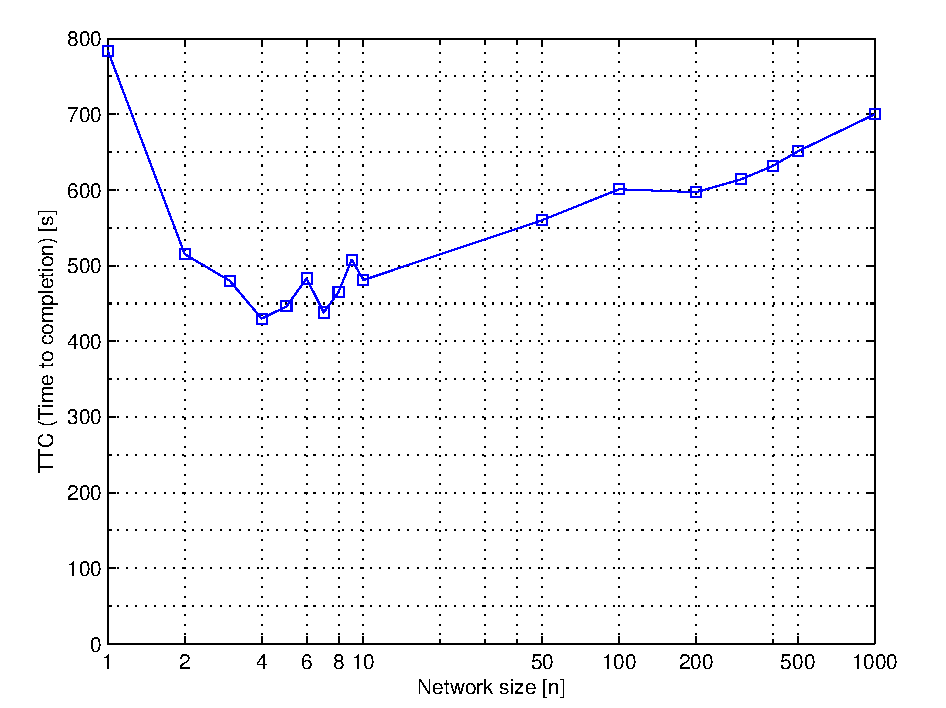
\includegraphics[width=0.49\textwidth]{figs/Experiment2_TTC}
  \caption{Time To Completion vs Network Size}
  \label{fig:network_size}
\end{figure}

From these results the following phenomena can be observed:

\paragraph{With a minimal number of peers the time to completion is highest.} This is because peers can only download one piece from the same seeder at any one time, so only a limited amount of work can be done in parallel in this case.

\paragraph{As more peers are added to the network time to completion reduces.} Adding more peers allows some work to be performed in parallel.

\paragraph{As number of peers steadily increases time to completion slowly increases.}
After the initial benefit of performing work in parallel, adding more peers results in more data that must be downloaded by all peers. The amount of data to be downloaded increases, but so does $\text{BW}_{\text{system}}$. The increase in $\text{BW}_{\text{system}}$ partially counteracts the increase in data to be downloaded, which is why the time to completion only increases slowly.

\subsection{Upload Bandwidth}
\label{subsec:upload_bandwidth_results}

The results presented by \fref{fig:upload_bandwidth_ttc} and \fref{fig:upload_bandwidth_ttransfer} were observed when varying $\text{BW}_{\text{up}}$ between 32-1024.

\begin{figure}[!htbp]
  \centering
  \includegraphics[width=0.49\textwidth]{figs/Experiment3_TTC}
  \caption{Time To Completion vs Upload Bandwidth}
  \label{fig:upload_bandwidth_ttc}
\end{figure}

\begin{figure}[!htbp]
  \centering
  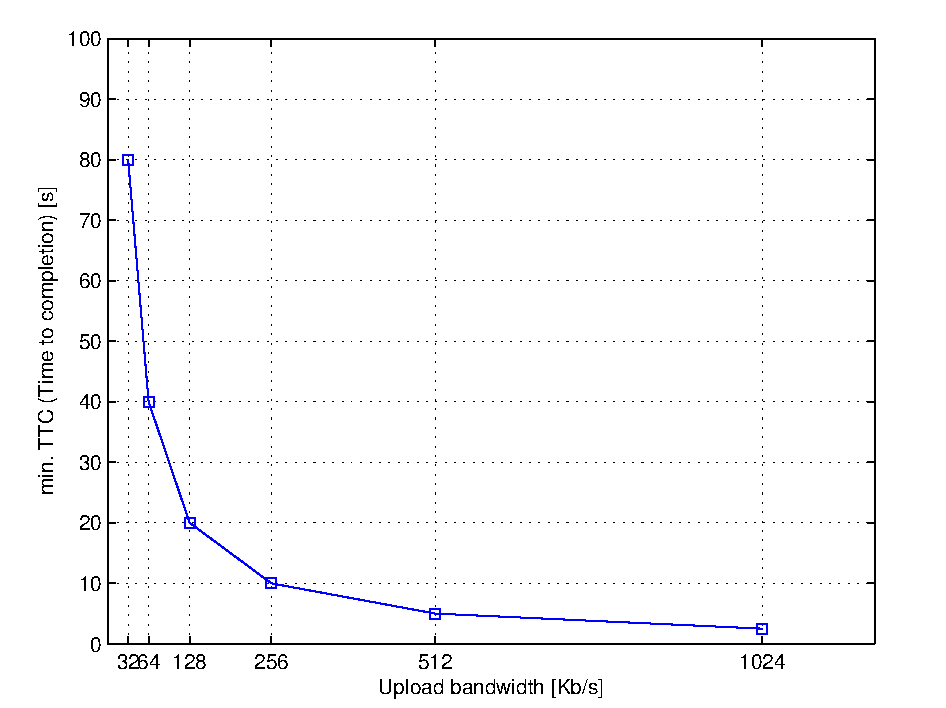
\includegraphics[width=0.49\textwidth]{figs/Experiment3_min_TTC}
  \caption{$T_{\text{transfer}}$ vs Upload Bandwidth}
  \label{fig:upload_bandwidth_ttransfer}
\end{figure}

From these results the following phenomena can be observed:

\paragraph{Time to completion improved most when $\text{BW}_{\text{up}}$ was raised from 32 to 64.}
When $\text{BW}_{\text{up}}$ is 32 $T_{\text{transfer}}$ is 80 time units (refer to \eref{eqn:t_transfer}). Obviously as $\text{BW}_{\text{up}}$ is doubled, $T_{\text{transfer}}$ will halve. Therefore, time to completion will improve as $\text{BW}_{\text{up}}$ is increased.

\paragraph{As $\text{BW}_{\text{up}}$ increases further, time to completion improves at a slower rate.}
The phenomenon of diminishing returns discussed earlier is applicable here also, so as $\text{BW}_{\text{up}}$ continues to increase $T_{\text{transfer}}$ accounts for less and less of the total bandwidth requirements, and $T_{\text{protocol}}$ starts to become the limiting factor. At this point, increasing $\text{BW}_{\text{up}}$ has a negligible effect on the time to completion.

\subsection{Piece Count}
\label{subsec:piece_count_results}

The results presented by \fref{fig:piece_count_ttc} and \fref{fig:piece_count_ttransfer} were observed when varying $\text{Count}_{\text{pieces}}$ between 1-50.

\begin{figure}[!htbp]
  \centering
  \includegraphics[width=0.49\textwidth]{figs/Experiment4_TTC}
  \caption{Time To Completion vs Piece Count}
  \label{fig:piece_count_ttc}
\end{figure}

From these results the following phenomena can be observed:

\paragraph{Time to completion is high when $\text{Count}_{\text{pieces}}$ is low.}
When $\text{Count}_{\text{pieces}}$ is low the process of disseminating pieces can not be parallelized very well. $T_{\text{transfer}}$ becomes higher so $\text{BW}_{\text{system}}$ increases at a slower rate. 
In this case, a peer can not begin seeding until it has a large percentage of the file.
Moreover, when $\text{Count}_{\text{pieces}}$ is low $\text{Util}_{\text{slots}}$ is likely to also be low (refer to \eref{eqn:utilization_slot}).

\paragraph{As $\text{Count}_{\text{pieces}}$ increases time to completion begins to decrease.}
When $\text{Count}_{\text{pieces}}$ increases $\text{Size}_{\text{pieces}}$ decreases. As a result $T_{\text{transfer}}$ decreases too and peers can begin seeding a given piece earlier. In other words $\text{BW}_{\text{system}}$ increases at a faster rate.
This leads to more work being performed in parallel because the file is broken down into more pieces. 
Consequently, peers can utilize their upload slots and upload bandwidth more efficiently.

\begin{figure}[!htbp]
  \centering
  \includegraphics[width=0.49\textwidth]{figs/Experiment4_min_TTC}
  \caption{$T_{\text{transfer}}$ vs Piece Count}
  \label{fig:piece_count_ttransfer}
\end{figure}

\paragraph{Increasing $\text{Count}_{\text{pieces}}$ too much has a negative effect.}
As $\text{Count}_{\text{pieces}}$ continues to increase $\text{Size}_{\text{piece}}$ becomes increasingly small, and $T_{\text{transfer}}$ accounts for less and less of the total bandwidth requirements. Again, we see that $T_{\text{protocol}}$ takes over as the major overhead.
At this point breaking the file into more pieces results in a measurable amount of additional protocol overhead, but has negligible benefits on $T_{\text{transfer}}$. The point of diminishing returns is reached and time to completion increases once again.

\subsection{Churn}
\label{subsec:churn_results}

An important fact that should be introduced here is that, to create churn the simulator must generate additional events that add/remove peers from the network. It takes a small amount of time to create each event and to increase the amount of churn the simulator must create more events. It is natural for an experiment with more churn to run for a longer duration, if for no other reason then simply because more events must be executed.

The results presented by \fref{fig:churn} were observed when varying the amount of churn between 0-70\%.

\begin{figure}[!htbp]
  \centering
  \includegraphics[width=0.49\textwidth]{figs/Experiment5_TTC}
  \caption{Time To Completion vs Churn}
  \label{fig:churn}
\end{figure}

From these results the following phenomena can be observed:

\paragraph{As expected, when there is no churn in the network time to completion is lowest.}
There are fewer events. Peers never fail or leave, so pieces are never lost and the amount of pieces in the system monotonically increases.

\paragraph{Time to completion increases quickly when churn is introduced.}
Amount of simulator events increases. The amount of pieces in the system is no longer guaranteed to monotonically increase. Furthermore, run time is dependent on which peers fail. If a failing peer is seeding any pieces, those pieces will be lost and $\text{BW}_{\text{system}}$ will also decrease.

\paragraph{Time to completion continues to increase as more churn is added.}
The amount of simulator events continues to increase. Due to the rise in number of failures, it is also increasingly likely that the number of pieces in the system will not monotonically increase, and the probability that failing peers are also seeding peers becomes higher.

An important observation of the results is that all live peers eventually become seeders. The reason for this is because the initial seeder is reliable (can never fail), all peers are guaranteed to eventually make progress.

\subsection{Leaving Seeders}
\label{subsec:leaving_seeders_results}

The results presented by \fref{fig:time_seeding} were observed when varying the amount of time peers remained in the network after seeding, between 0-500ms.

\begin{figure}[!htbp]
  \centering
  \includegraphics[width=0.49\textwidth]{figs/Experiment6_PIECES}
  \caption{Available Pieces vs Time Seeding}
  \label{fig:time_seeding}
\end{figure}

From these results the following phenomena can be observed:

\paragraph{When peers seed for a minimal amount of time, some peers never become seeders.} Seeders leave before every piece can be disseminated to some other peer.

\paragraph{As time spent seeding increases, the remaining peers are able to download more pieces.} Some peers still never download the entire file. Seeders leave before every piece can be disseminated to some other peer. 
However, the longer a seeder stays the more unique pieces will be disseminated. For all peers to eventually become seeders it is important that every piece is sufficiently replicated in the network.

\paragraph{Once time spent seeding surpasses a threshold (300 time units), all peers become seeders.} All peers are able to eventually acquire all pieces and become seeders.
Simply put, seeders must stay in the network long enough to ensure every piece is replicated sufficiently such that every piece disseminates throughout the network to enough peers to guaranty that when seeders leave, no pieces become unattainable.

\section{Discussion}
\label{sec:discussion}
Despite Basic Torrent's relative simplicity, while carrying out this project various interesting phenomena were discovered. 
These were documented, reasoned about, and used to incrementally build theories and understanding of the protocol. 

Most findings were significantly more complex than they initially appeared, and many phenomena proved to be multi-dimensional and difficult or impossible to explain with relation to only one variable.

The goal of this report was to introduce a simplified version of BitTorrent.
The protocol was not intended for practical use, but rather for use in analyzing phenomena that arise in peer-to-peer systems like BitTorrent. 
To that end, creating and experimenting with Basic Torrent has been worthwhile.

\begin{flushright}
$\blacksquare$
\end{flushright}

\end{document}
